\chapter{Prefix - Suffix Product}
\section{Questions}\\


\href{https://leetcode.com/problems/product-of-array-except-self/description/}{238. Product of Array Except Self}


\section{Example Usage}\\



\begin{lstlisting}
 public int[] ProductExceptSelf(int[] nums) {
        var prefix = new int[nums.Length];
        var suffix = new int[nums.Length];
        var result = new int[nums.Length];

				prefix[0]=1;
        for(int i = 1; i<nums.Length; i++){
					prefix[i]=prefix[i-1]*nums[i-1];
        }


        suffix[nums.Length-1]=1;

        for(int j=nums.Length-2; j>= 0; j--){
            suffix[j]=suffix[j+1] * nums[j+1];
        }


        for(int i = 0; i<nums.Length; i++){
            result[i] = prefix[i]*suffix[i];
        }
        return result;
    }
		
\begin{figure}
		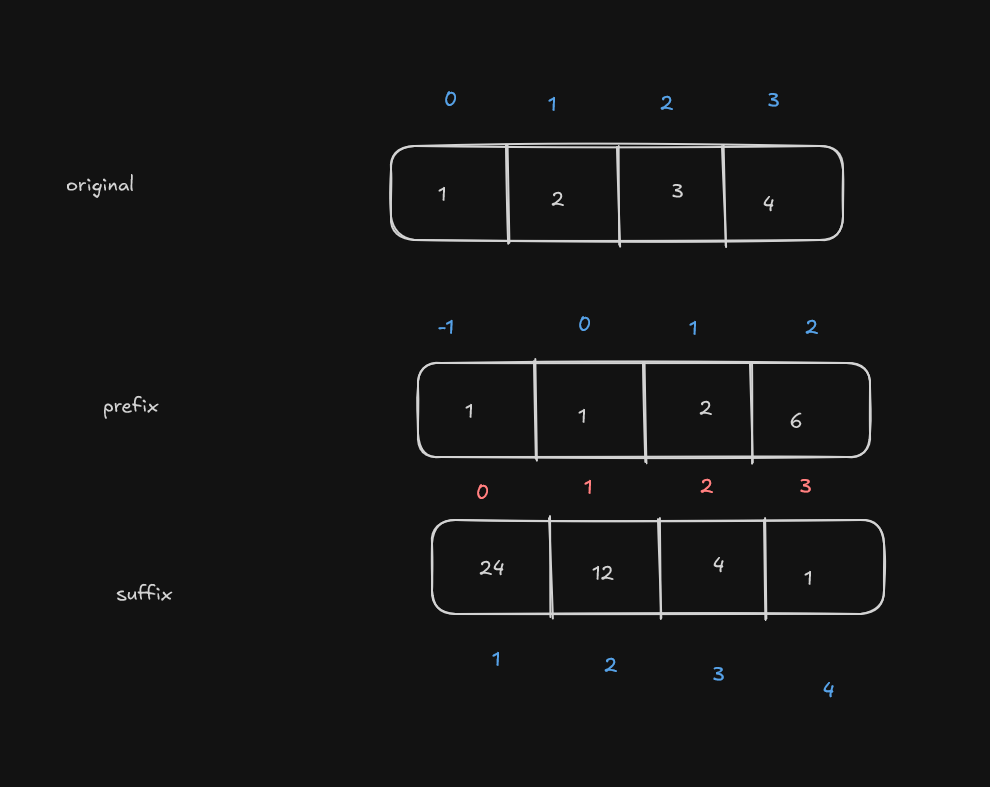
\includegraphics{1.png}
\end{figure}

\begin{figure}
		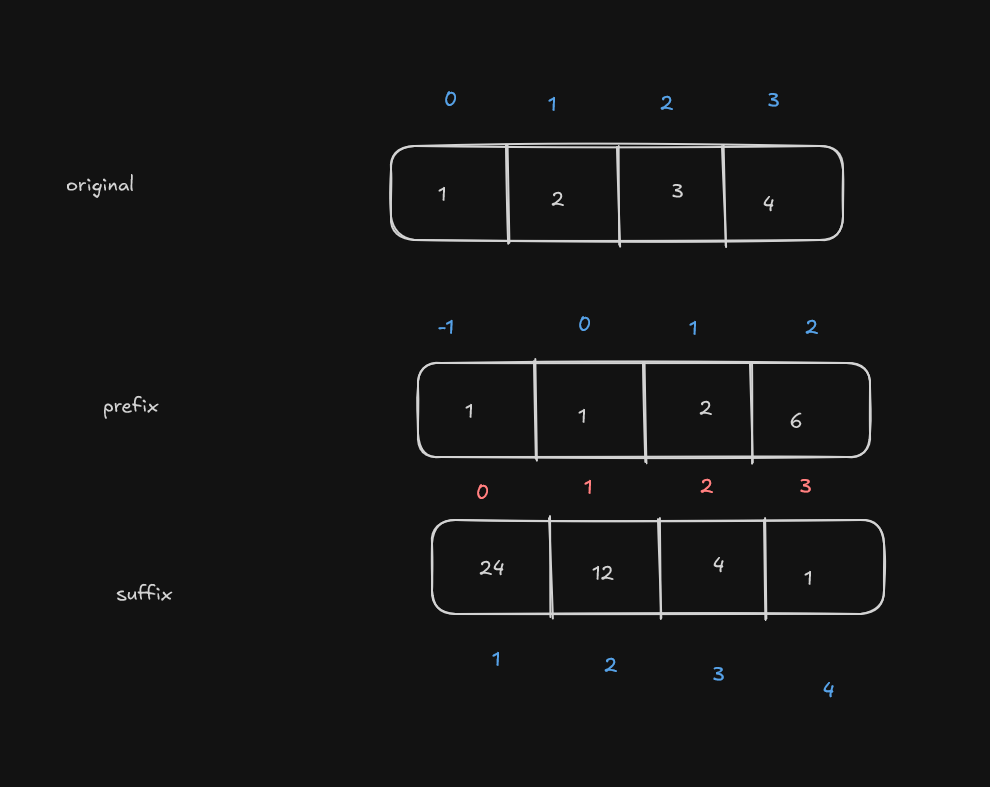
\includegraphics{1.eps}
\end{figure}

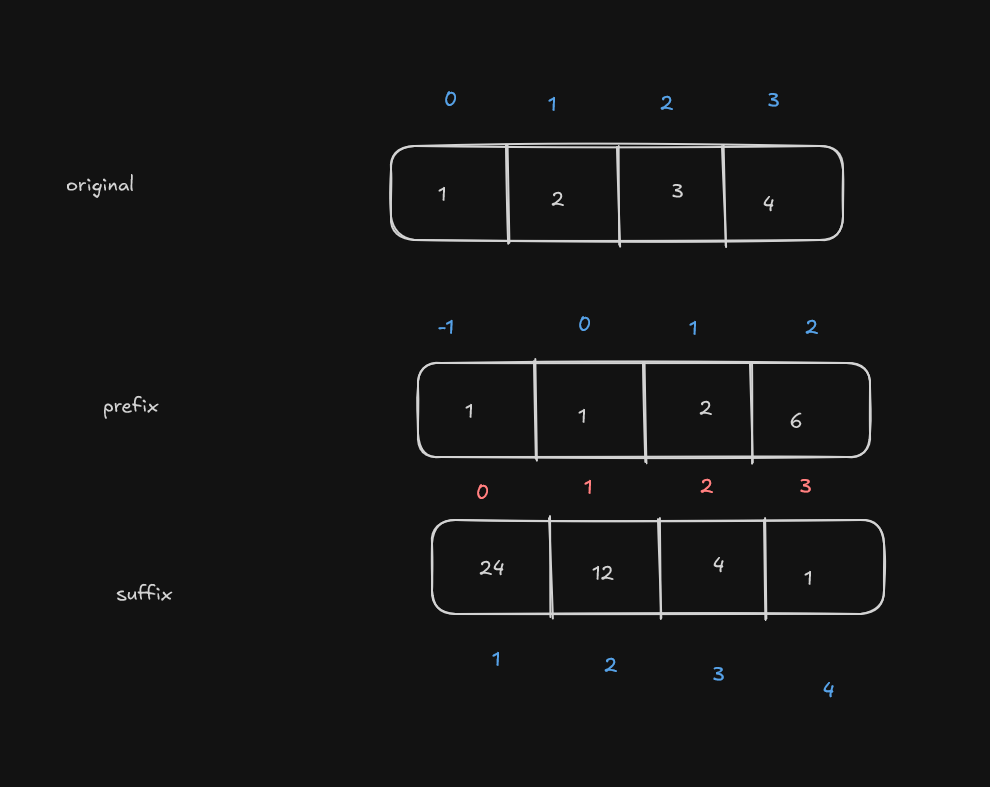
\includegraphics{1.eps}

\end{lstlisting}\\ \\